% Authors: Tony Li
% Emails: songli@berkeley.edu

\qns{Thevenin's and Norton's Equivalent Circuit}

In this set, we will review two useful theorems that you might have learned in previous physics classes.
\textbf{Thevenin's Theorem} states that we can replace entire network by an equivalent circuit that contains only
an independent voltage source in series with an impedance (resistor) such that the current-voltage 
relationship at the load is unchanged.
\begin{figure}[H]
  \centering
  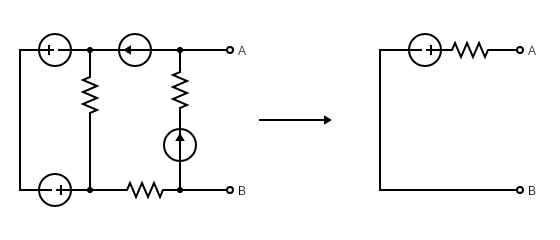
\includegraphics[scale=0.4]{\bank/Thevenin/Figures/thevenin.png}
  \caption{Thevenin's Equivalent Circuit}
  \label{A Thevenin Equivalent Circuit Example}
\end{figure}
As shown above, we have a linear electrical network, containing only voltage sources, curretn sources, resistors, and
two terminals A and B. The circuit can be always transformed to an equivalent circuit with only one voltage source, one resistor,
and two terminals A and B. By using this theorem, we can largely simplfy the circuit. A more easier way to understand this is that
we can use a black box to include everything connecting to two terminals, and then replace the black box with a voltage source and 
a resistor in series. 

\textbf{Norton's Thereom} is identical to Thevenin's Theorem except that the equivalent circuit is an
independent current source in parallel with an impedance (resistor). Therefore, the Norton equivalent circuit 
is a source transformation of the Thevenin equivalent circuit.
\begin{figure}[H]
  \centering
  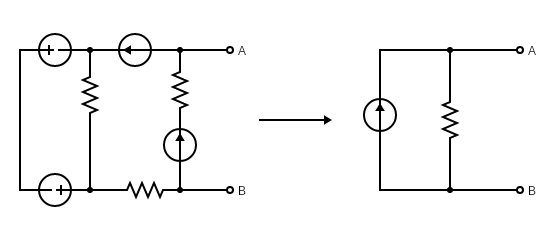
\includegraphics[scale=0.4]{\bank/Thevenin/Figures/norton.png}
  \caption{Norton's Equivalent Circuit}
  \label{A Norton Equivalent Circuit Example}
\end{figure}
Quite similar to Thevenin's theorem, we can replace a linear electrical network with a current source and a resistor in parallel.

Note that, the power source can be non-constant, which means that we could have an AC circuit. As a result, we need to use
impedances at a given frequency substituting the resistances.

How to find out the voltage and resistance in the equivalent circuit:
First, let's assume that the voltage source is ideal and does not have any internal resistance. In a non-ideal case, we need 
to add one more resistor beside the voltage source to represent the internal resistance of the voltage source. However, for an ideal 
current source, it has infinite internal resistance, 
Then use KVL, KCL, and Ohm's Law to find out the resistance and voltage in the Thevenin's quivalent circuit. Similar procdure
also applies to the Norton's equivalent circuit.

For the following problems, we will first try to obtain the Thevenin's equivalent circuit of the following circuit.
\begin{figure}[H]
  \centering
  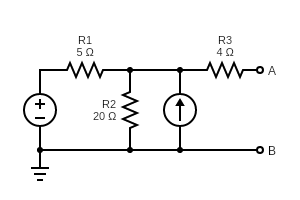
\includegraphics[scale=0.7]{\bank/Thevenin/Figures/circuit_problem.png}
  \caption{Voltage of the voltage source $V_s$ is 25V, and the current of the current source $I_s$ is 3A.}
  \label{A Circuit problem}
\end{figure}

\begin{enumerate}
  % Part(a)
  \qitem 
   First, we need to create an imaginary wire connecting to terminal A and B, and also a terminal C.
   \begin{figure}[H]
    \centering
    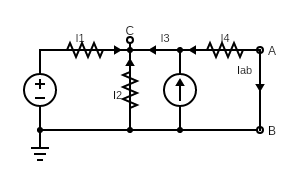
\includegraphics[scale=0.7]{\bank/Thevenin/Figures/circuit1.png}
    \caption{The imaginary current is flowing from A to B with the magnitude $I_{ab}.$}
    \label{A Circuit problem}
  \end{figure}
  Denote the voltage at terminal C as $V_c$. What are the magnitudes of the currents $I_1$, $I_2$, $I_3$, $I_4$?
  By using KCL, can you derive an equation including all four currents?

  \meta {
    Please ask students why it is important to use KCL? How do we know that by using KCL we can get the value of $V_c$?
    $I_2$ is negative because the direction of the current $I_2$ is from ground to terminal C. It does not mean that the magnitude
    of $I_2$ is negative. In KCL, whether the current is negative or postive is determined by its direction.
  }

  \sol{
    $I_1 = \frac{V_s-V_c}{R_1}=\frac{25V-V_c}{5\Omega}$, by Ohm's Law.
    \newline $I_2 = \frac{V_{ground}-V_c}{R_2}=\frac{0V-V_c}{20\Omega}=\frac{-V_c}{20\Omega}$, by Ohm's Law. 
    \newline $I_3 = I_s + I_4=3A+I_4$, by KCL.
    \newline Because we have created a wire from terminal A to B, terminal A is grounded now.
    $I_4=\frac{V_{ground}-V_c}{R_3}=\frac{-V_c}{4\Omega}$.
    \newline $I_1+I_2+I_3=0\Rightarrow{\frac{25-V_c}{5\Omega}-\frac{V_C}{20\Omega}+3A+I_4=0}$.
    \newline The simplified equation should be $8-\frac{V_c}{2}=0\Rightarrow{V_c=16V}$.
  }

  % Part(b)
  \qitem After establishing the equation, you should be able to find out $V_c$. Based on the value of $V_C$, what is the
  magnitude of $I_{ab}$? $I_{ab}$ is called short-circuit current, it is the current that actually flow from A to B if you connect
  two terminals in the equivalent circuit.

  \sol {
    Apply KCL at terminal A, and we get $I_{ab}=I_4=\frac{V_c-V_{ground}}{R_3}=\frac{16V}{4\Omega}=4A$.
  }

  %part c
  \qitem Then, suppose that there is \textbf{no such imaginary wire across A and B}. Let's focus on finding the value of the \textbf{Thevenin Equivalent Resistance} $R_e$. 
  To calculate the Thevenin equivalent resistance, remove all power sources from the original circuit. The voltage
  sources are short-circuited and current sources are opened. What is $R_e$, the total resistance between terminal A and B in the remaining circuit?
  \newline\emph{Hint:} The remaining circuit now only has three resistors. $R_1$ and $R_2$ are now in parallel and $R_3$
  is in series with $R_1$ and $R_2$. 
  \begin{figure}[H]
    \centering
    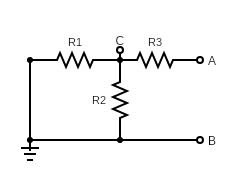
\includegraphics[scale=0.7]{\bank/Thevenin/Figures/circuit4.png}
    \caption{The remaining circuit, and the total resistance between A and B is $R_e$.}
    \label{A Circuit problem}
  \end{figure}
  \meta {
    We need the imaginary wire to calculate the shor-circuit current $I_{ab}$ in Thevenin's equivalent circuit. Now, deleting that wire helps us to
    find out the total resistance between A and B $R_e$. Why is the voltage source like a wire and the current
    source like an opne-circuit? Because we are using ideal power sources, and the voltage source has no internal resistance and the current source has 
    the infinite internal resistance. 
  }
  \sol {
    Now the voltage source acts like a wire, and the total resistance between C and B is 
    $\frac{1}{\frac{1}{R_1}+\frac{1}{R_2}}=\frac{1}{\frac{1}{5\Omega}+\frac{1}{2o\Omega}}=4\Omega$.
    Thus, the total resistance between A and B is $R_e=4\Omega+R_3=8\Omega$.
  }

  % Part(d)
  \qitem We are almost done! Now, it's time to draw our Thevenin's equivalent circuit.
  \begin{figure}[H]
    \centering
    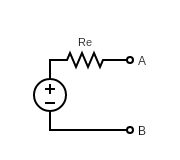
\includegraphics[scale=0.7]{\bank/Thevenin/Figures/circuit2.png}
    \caption{The voltage source has voltage $V_e$ and the resistor has the resistance $R_e$.}
    \label{A Circuit problem}
  \end{figure}
  What are the values of $V_e$ and $R_e$?
  \newline\emph{Hint:} What law should we use to get $V_e$? Remember $I_{ab}$ is the short-circuit current.

  \meta {
    Please explain thoroughly why we need the imaginary current at the first place. If we want to get $V_e$ in the equivalent circuit, 
    we need to connect two terminals first in the equivalent cicuit, and then apply the Ohm's Law.
  }
  \sol{
    $R_e$ is just what we have found previously $8\Omega$. 
    $V_e=R_e*I_{ab}=8\Omega*4A=32V$, by Ohm's Law.
  }
  \end{enumerate}

  Now we know how to get a Thevenin's Equivalent Circuit, but how do we get a Norton's Equivalent Circuit? 
  In this question we will look at how to use Thevenin's Circuit to get the Norton's Circuit.
  \begin{enumerate}[resume]
  % Part(e)
  \qitem Let's look at the same graph, Figure 3. You have already obtained the value of the short-circuit current $I_{ab}$ and 
  the total resistance $R_e$ between the terminal A and B. Why don't we just use both of the values to find out $I_e$ and $R_e$ in the Norton's equivalent circuit shown below?
  \begin{figure}[H]
    \centering
    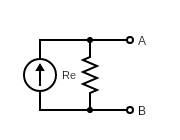
\includegraphics[scale=0.7]{\bank/Thevenin/Figures/circuit3.png}
    \caption{The current source has current $I_e$ and the resistor has the resistance $R_e$.}
    \label{A Circuit problem}
  \end{figure}
  \meta {
    Expain that why we can use the same data we got previously. We can still apply the Ohm's Law to get $I_e$ and $R_e$.
  }
  \sol {
    $R_e$ in Norton is equal to $R_e$ in Thevenin for the same circuit, becasue if you consider the current source has an open-circuit,
    $R_e$ in Norton is also the total resistance between terminal A and B.
    \newline $R_e=8\Omega$ and $I_e=\frac{V_{ab}}{R_e}= \frac{32V}{8\Omega}=4A$.
    \newline Two helpful properties of Thevenin and Norton Conversion:
    \newline 1. Thevenin resistance and Norton resistance are equal.
    \newline 2. Thevenin voltage is equal to the Norton current times the Norton resistance.
  }

\end{enumerate}
